% !TeX encoding = UTF-8
\documentclass{sysuthesis}

% 设置论文的基本信息,包括题目、作者、专业、导师、学院、摘要和关键词等必要信息
% !TEX root = ./main.tex
% 设置论文题目,第一个“{}”为中文题目,第二个“{}“为英文题目
\title{中山大学研究生学位论文\LaTeX{}非官方模版}
{English Title for Sun Yat-sen University Thesis \LaTeX{} Unofficial Template}

% 设置作者,第一个“{}”为中文名字,第二个“{}“为英文名字
\author{张三}{Zhang San}

% 设置专业,第一个“{}”为中文专业名,第二个“{}“为英文专业名
\major{天体物理}{Astrophysics}

% 设置指导教师,第一个“{}”为中文名字,第二个“{}“为英文名字
\supervisor{李四}{Li Si}

% 设置学位名
\degree{硕士}

% 设置关键词,第一个“{}”为中文关键词,第二个“{}“为英文关键词
\keywords{天体物理、引力波、黑洞}{Astrophysics, Gravitational Wave, Black Holes}

% 设置学院
\school{物理与天文学院}

% 设置校区
\campus{珠海}

% 设置日期,默认是当天时间,具体到日
\date{2022年6月}

% 设置新的latex命令
\newcommand{\dd}{\mathrm{d}}
% 调用的宏包
\usepackage{longtable}
\usepackage{tablefootnote}
\usepackage{hologo}


\begin{document}

% 前置部分
\frontmatter

% 扉页
\maketitle

% 原创性及使用授权说明
\copyrightpage

% 中英文摘要
% !TEX root = ../main.tex
% 中英文摘要
\begin{abszh}
    摘要概括论文的主要信息,包括研究目的、方法、成果及最终结论。硕士论文摘要一般不超过1200字。博士论文摘要一般不超过2000字。关键词是供检索用的主题词条,应采用能覆盖论文主要内容的通用词。关键词一般列3~5个。

    摘要概括论文的主要信息,包括研究目的、方法、成果及最终结论。硕士论文摘要一般不超过1200字。博士论文摘要一般不超过2000字。关键词是供检索用的主题词条,应采用能覆盖论文主要内容的通用词。关键词一般列3~5个。
\end{abszh}

% 英文摘要
\begin{absen}
    The first paragraph: The abstract summarizes the main information of the paper, including the purpose, methodology, results and final conclusions of the study. The abstract of the master's thesis generally does not exceed 1200 words. The abstract of the PhD thesis generally does not exceed 2000 words. Keywords are the subject terms for searching, and generic words that cover the main content of the paper should be used. Keywords generally list 3 to 5.
    
    The second paragraph: The abstract summarizes the main information of the paper, including the purpose, methodology, results and final conclusions of the study. The abstract of the master's thesis generally does not exceed 1200 words. The abstract of the PhD thesis generally does not exceed 2000 words. Keywords are the subject terms for searching, and generic words that cover the main content of the paper should be used. Keywords generally list 3 to 5.
\end{absen}

% 目录
\tableofcontents

% 插图索引
\listoffigures

% 表格索引
\listoftables

% 主体部分
\mainmatter

% 正文
% !TEX root = ../main.tex
\chapter{前言}

\blfootnote{\copyright\ \number\year\ \href{https://github.com/yanghw8}{yanghw8}}
\blfootnote{更新时间:\today}

\sysuthesis{}是旨在为中山大学熟悉\LaTeX{}语言的研究生提供一个方便易用的学位论文写作模版,其设置的排版格式力求尽可能符合《\href{https://sysgraduate.sysu.edu.cn/sites/graduate.prod.dpcms4.sysu.edu.cn/files/2019-04/%E4%B8%AD%E5%B1%B1%E5%A4%A7%E5%AD%A6%E7%A0%94%E7%A9%B6%E7%94%9F%E5%AD%A6%E4%BD%8D%E8%AE%BA%E6%96%87%E6%A0%BC%E5%BC%8F%E8%A6%81%E6%B1%82.pdf}{中山大学研究生学位论文格式要求}》。首先声明:\strong{本模版不是官方模版,无法保证它完全符合学校的相关要求,在开始使用前,您同意,任何由于本模板而引起的论文格式审查问题与本模板作者无关。}

本模版暂时没有为本科生学位论文设置格式,如果您是本科生,请移步至\href{https://github.com/SYSU-SCC/sysu-thesis}{本科生模版}。如果您没有接触过\LaTeX{},又不打算花费时间和精力来入门,推荐您使用Microsoft Office套装来编写您的学位论文。如果您是\LaTeX{}语言的初学者,那么希望以下内容会对您的学习有所帮助。

\section{模版文件结构}

本模版仅支持\hologo{XeTeX}排版引擎,其相应的编译器称为“xelatex”,字符编码仅支持UTF-8,进行编译时,您需要使用正确编译器。本模版需要编译的主文件为\texttt{main.tex},在编译时请选择“xelatex”编译器,由于是中文文档并且与\hologo{BibTeX}配合使用,请遵从以下编译步骤:
\begin{itemize}
    \item xelatex
    \item bibtex
    \item xelatex
    \item xelatex
\end{itemize}
如此您将得到一个最终完成的PDF文件。

本模版的文件目录结构见\ref{fig:dir}。重要的文件为\texttt{sysuthesis.cls},\texttt{sysuthesis.bst},分别是设置了本模版的论文排版格式和参考文献引用格式,在使用时,请您不要轻易修改这两个文件。您可以编辑的文件有:
\begin{itemize}
    \item \texttt{setup.tex}文件:编辑您的论文题目、作者姓名、专业、指导教师、关键词和学院及日期等关键信息,设置用于本文档的新\LaTeX{}命令以及调用的宏包;
    \item \texttt{contents}文件夹里面的文件:将您的文章内容分为多个部分编辑好,并在\texttt{main.tex}中导入并排好顺序;
    \item \texttt{ref}文件夹里的\texttt{refs.bib}文件:用于编辑您的引用文献信息,请遵从hologo{BibTeX}的语法格式,以免达成意料之外的效果;
    \item 为了方便起见,请将您的要使用的图片和代码文件放到相应的文件夹,以免造成不必要的混乱。
\end{itemize}

\begin{figure}[!htp]
    \centering
    \begin{forest}
        directory,
        [sysuthesis-unoffical,  label=right:{\zihao{5}主目录}
          [codes, label=right:{\zihao{5}代码文件夹}
            [cohere.py, label=right:{\zihao{5}代码环境示例Python代码}]
          ]
          [contents, label=right:{\zihao{5}主要\TeX{}文件的文件夹}
            [abstract.tex, label=right:{\zihao{5}摘要内容编辑}]
            [ack.tex, label=right:{\zihao{5}后记内容编辑}]
            [appendix.tex, label=right:{\zihao{5}附录内容编辑}]
            [chapter1.tex]
            [chapter2.tex]
            [chapter3.tex]
            [summary.tex, label=right:{\zihao{5}结语内容编辑}]
          ]
          [figures, label=right:{\zihao{5}图片文件夹}
            [hexbin.pdf]
            [histogram.pdf]
            [piechart.pdf]
            [sysu.pdf]
          ]
          [ref, label=right:{\zihao{5}放置引用文献信息的文件的文件夹}
            [refs.bib, label=right:{\zihao{5}文件的语法格式应为\hologo{BibTeX}格式}]
          ]
          [main.tex, label=right:\strong{\zihao{5}需要编译的主\TeX{}文件}]
          [main.pdf, label=right:{\zihao{5}编译生成的PDF文件}]
          [README.md]
          [setup.tex, label=right:{\zihao{5}配置论文信息、设置新命令以及调用宏包的文件}]
          [sysuthesis.bst, label=right:{\zihao{5}设置参考文献格式的文件}]
          [sysuthesis.cls, label=right:{\zihao{5}设置论文排版格式的类文档}]
        ]
    \end{forest}
    \caption{本模版的文件目录}
    \label{fig:dir}
\end{figure}

\section{\TeX{} Live套装及其他软件}

\TeX{} Live是由国际\TeX{}用户组(\TeX{} Users Group,TUG)整理和发布的\TeX{}软件套装,包含与\TeX{}系统相关的各种程序、编辑与查看工具、常用宏包及文档、常用字体及多国语言支持。

\subsection{软件下载及安装}

\TeX{} Live支持大家主要使用的Unix/Linux、Windows以及Mac OS等操作系统,它保持着每年一版的更新频率,是开源软件。可以直接到\href{https://www.tug.org}{\strong{TUG}}官网下载\href{https://www.tug.org/texlive}{\TeX{} Live},但可能受国内防火墙限制了下载速度,推荐大家到\href{https://mirrors.tuna.tsinghua.edu.cn/CTAN/}{清华大学开源软件镜像站}下载。请注意,对于Mac OS 系统,请选择下载\strong{Mac\TeX{}}。下载完成后,请根据提示进行安装,一般都是一路默认安装。

\subsection{\LaTeX{}编辑器}

\LaTeX{}编辑器一般都会随着套件一起安装下来,如果你觉得默认的编辑器用起来不方便,下面推荐几个\LaTeX{}编辑器。

\begin{itemize}
    \item Visual Studio Code:这是一款由微软开发且跨平台的免费源代码编辑器。该软件支持语法高亮、代码自动补全、代码重构功能,默认支持非常多的编程语言。而且有内置的扩展程序商店,可以下载扩展支持你所需要的语言插件,\strong{需要配置环境}。请到\url{https://code.visualstudio.com}下载。
    \item Overleaf:这是一款\strong{在线协作}的\LaTeX{}编辑器,与很大科学杂志出版商有合作关系,上面不但提供官方期刊的\LaTeX{}模板,还能直接将文件提交至这些出版社。官方网站为\url{https://www.overleaf.com}。
    \item TeXstudio:这是一款开源的跨平台\LaTeX{}编辑软件,支持交互式拼写检查、代码折叠、语法高亮等特性。官网网站为\url{http://texstudio.sourceforge.net}。
\end{itemize}

\subsubsection{相关配置}

各种\LaTeX{}编辑器的配置可以轻易在网上找到,而且有的都比较简单。下面只介绍Visual Studio Code的配置。
\begin{itemize}
    \item 在扩展商店里找到\strong{LaTeX Workshop}插件,点击安装;
    \item 找到扩展设置(Extension Settings),找到\texttt{settings.json}文件,编辑它,在里面加入你的配置代码。以下是我的配置:
\begin{lstlisting}
    "latex-workshop.latex.tools": [
        {
            "name": "xelatex",
            "command": "xelatex",
            "args": [
                "-synctex=1",
                "-interaction=nonstopmode",
                "-file-line-error",
                "%DOCFILE%"
            ]
        },
        {
            "name": "pdflatex",
            "command": "pdflatex",
            "args": [
                "-synctex=1",
                "-interaction=nonstopmode",
                "-file-line-error",
                "%DOCFILE%"
            ]
        },
        {
            "name": "latexmk",
            "command": "latexmk",
            "args": [
                "-synctex=1",
                "-interaction=nonstopmode",
                "-file-line-error",
                "-pdf",
                "-outdir=%OUTDIR%",
                "%DOCFILE%"
            ]
        },
        {
            "name": "bibtex",
            "command": "bibtex",
            "args": [
                "%DOCFILE%"
            ]
        }
    ],
    "latex-workshop.latex.recipes": [
        {
            "name": "XeLaTeX",
            "tools": [
                "xelatex"
            ]
        },
        {
            "name": "PDFLaTeX",
            "tools": [
                "pdflatex"
            ]
        },
        {
            "name": "BibTeX",
            "tools": [
                "bibtex"
            ]
        },
        {
            "name": "LaTeXmk",
            "tools": [
                "latexmk"
            ]
        },
        {
            "name": "xelatex -> bibtex -> xelatex*2",
            "tools": [
                "xelatex",
                "bibtex",
                "xelatex",
                "xelatex"
            ]
        },
        {
            "name": "pdflatex -> bibtex -> pdflatex*2",
            "tools": [
                "pdflatex",
                "bibtex",
                "pdflatex",
                "pdflatex"
            ]
        }
    ],
    "latex-workshop.view.pdf.viewer": "tab",
    "latex-workshop.bind.altKeymap.enabled": true,    
\end{lstlisting}
    \item 之后可以在\TeX{}环境里,选择对应的\strong{Build LaTeX project}进行编译。
\end{itemize}

\section{推荐读物}

本文档不是\LaTeX{}的入门教程,因此不会对复杂的\LaTeX{}代码进行介绍。如果您只是用来编写您的学位论文,完全可以将源代码里的内容替换成你的内容,然后经过若干次复制、粘贴和修改,最终您会得到你所需要的文档。然而,有时候您想实现一些自己的个性化内容,希望下面推荐的读物可以帮助到您:
\begin{itemize}
    \item \href{https://www.overleaf.com/learn}{Overleaf:Documentation},在线英文文档,在里面实现不同功能的\LaTeX{}示例应有尽有;
    \item \href{http://www.ptep-online.com/ctan/lshort_chinese.pdf}{《一份不太简短的\hologo{LaTeX2e}介绍》};
    \item \href{https://github.com/wklchris/Note-by-LaTeX}{《简单粗暴\LaTeX{}》};
    \item 刘海洋:《\LaTeX{}入门》\cite{Liu:2013latexrm}。
\end{itemize}
最后祝您使用愉快!
% !TEX root = ../main.tex
\chapter{标题及字体示例}

\section{二级标题}

\subsection{三级标题}

\subsubsection{四级标题}

\section{字体示例}

\subsection{中文字体}

\begin{center}

    {\zihao{2}\heiti 二号黑体居中}

    {\zihao{-2}\heiti 小二号黑体居中}

    {\zihao{3}\heiti 三号黑体居中}

    {\zihao{-3}
        {\heiti 小三号黑体居中}

        {\songti 小三号宋体居中}

        {\bfseries\songti 小三号宋体加粗居中}
    }

    {\zihao{4}
        {\heiti 四号黑体居中}

        {\songti 四号宋体居中}

        {\bfseries\songti 四号宋体加粗居中}
    }
    
    {\zihao{-4}
        {\songti 小四号宋体居中}

        {\bfseries\songti 小四号宋体加粗居中}

        {\kaishu 小四号楷书居中}

        {\lishu 小四号隶书居中}
    }

    {\songti\zihao{5} 宋体五号居中}

\end{center}

\subsection{西文字体}

\subsubsection{正文字体:Times New Roman}
请直接使用,或通过\texttt{$\backslash$texttt}命令来使用:

ABCDEFGHJKLMNOPQRSTUVWXYZ 

abcdefghjklmnopqrstuvwxyz 

1234567890

\subsubsection{斜体:Times New Roman Italic}
请通过\texttt{$\backslash$textit}命令来使用:

\textit{ABCDEFGHJKLMNOPQRSTUVWXYZ}

\textit{abcdefghjklmnopqrstuvwxyz}

\textit{1234567890}

\subsubsection{无衬线字体:\textsf{Helvetica}}
请通过\texttt{$\backslash$textsf}命令来使用:

\textsf{ABCDEFGHJKLMNOPQRSTUVWXYZ}

\textsf{abcdefghjklmnopqrstuvwxyz}

\textsf{1234567890}

\subsubsection{等宽字体:\texttt{Monaco}}
请通过\texttt{$\backslash$texttt}命令来使用:

\texttt{ABCDEFGHJKLMNOPQRSTUVWXYZ}

\texttt{abcdefghjklmnopqrstuvwxyz}

\texttt{1234567890}

\subsection{数学符号}
数学符号只能在$\$\quad\$$限定域或如\texttt{align}等数学模式(math mode)中使用。

\subsubsection{数学符号为英文字母及阿拉伯数字}
$ABCDEFGHJKLMNOPQRSTUVWXYZ$

$abcdefghjklmnopqrstuvwxyz$

$1234567890$

\subsubsection{希腊字母}
$\alpha\beta\gamma\delta\epsilon\varepsilon\zeta\eta\theta\vartheta\iota\kappa\lambda\mu\nu\xi o\pi\varpi\rho\varrho\sigma\varsigma\tau\upsilon\phi\varphi\chi\omega$

$\Gamma\Delta\Theta\Lambda\Xi\Pi\Sigma\Upsilon\Phi\Psi\Omega$

\subsubsection{其他数学符号}
\begin{align*}
    \sum, \quad \prod, \quad \int, \quad, \oint, \quad \bigcap, \quad \bigcup, \quad \bigodot, \quad \bigotimes, \quad \bigoplus
\end{align*}

更多特殊符号的\LaTeX{}命令见\href{https://mirrors.ustc.edu.cn/CTAN/info/symbols/comprehensive/symbols-a4.pdf}{The Great, Big List of LATEX Symbols}。

    


\section{格式内容}

主体部分包括引言(前言),国内外文献综述,正文,结语,参考文献。要求图表清晰,叙述流畅,章节有序,层次分明。

引言(前言)部分内容主要为本研究课题的学术背景及理论与实际意义;本研究课题的来源及主要研究内容;建立研究的线索与思路。

\subsection{格式说明}

\subsubsection{说明一}

文中的公式、插图、表格等,一律用阿拉伯数字按章顺序编号。如\ref{fig:hexbin}、    \ref{tab:01}、\ref{eqn:taylorseries}等。图序及图名置于图的下方,居中排列;表序及表名置于表的上方,居中排列。

\subsubsection{说明二}

章、节、条的编排为章居中,节左边空二格排版。内文文字排版的字体、字号、行距、字距以版面清晰、容易辨识和阅读为原则,一般可参照下面要求进行排版:章的题名建议采用小二号黑体,居中;节的题名建议采用小三号宋体,加粗,左起空两格;文章段落内容建议采用小四号宋体。

% !TEX root = ../main.tex
\chapter{一些重要的\LaTeX{}环境}\label{chap:evm}

本模版中的公式、插图、表格和章节等,均用\texttt{$\backslash$lable\{<key>\}}来在\LaTeX{}代码中标记位置,用\texttt{$\backslash$ref\{<key>\}}来在代码中引用,其中\texttt{<key>}为自定义的标签。

\section{公式示例}

文中的公式建议使用\texttt{amsmath}宏包的\texttt{align}环境,该环境在对多行公式对齐方面具有很大的优势,具体的讨论请看知乎用户\href{https://www.zhihu.com/people/bo-xue-duo-wen-63}{\strong{博闻多学}}的\href{https://www.zhihu.com/question/477805692/answer/2045084752}{\strong{回答}}。

下面进行公式示例。普通公式:
\begin{align}
    a+b=x.
\end{align}
带有积分和分隔的公式:
\begin{align}
   \int^{\infty}_{0} f(x)\dd{x}, \qquad \oint_{C} f(z)\dd {z}.
\end{align}
多行公式:
\begin{align}
    \left(1+x\right)^{\alpha} &= \sum^{\infty}_{n=0}\left(\begin{matrix} \alpha \\ n\end{matrix}\right)x^n \nonumber \\ 
    &= 1 + \alpha x + \frac{\alpha(\alpha-1)}{2!}x^2 + \cdots + \frac{\alpha(\alpha-1)\cdots(\alpha-n+1)}{n!} + \cdots
    \label{eqn:taylorseries}
\end{align}
这里注意,对不需要编号的行要取消公式编号,即要在该行公式的源代码后边使用\texttt{$\backslash$nonumber}命令。

公式的引用示例:\ref{eqn:taylorseries}为泰勒级数。

\section{插图示例}

文中插图的插图建议使用\texttt{graphicx}宏包的\texttt{figure}环境搭配\texttt{$\backslash$includegraphics}命令。例如:
\begin{figure}[!htp]
	\centering
	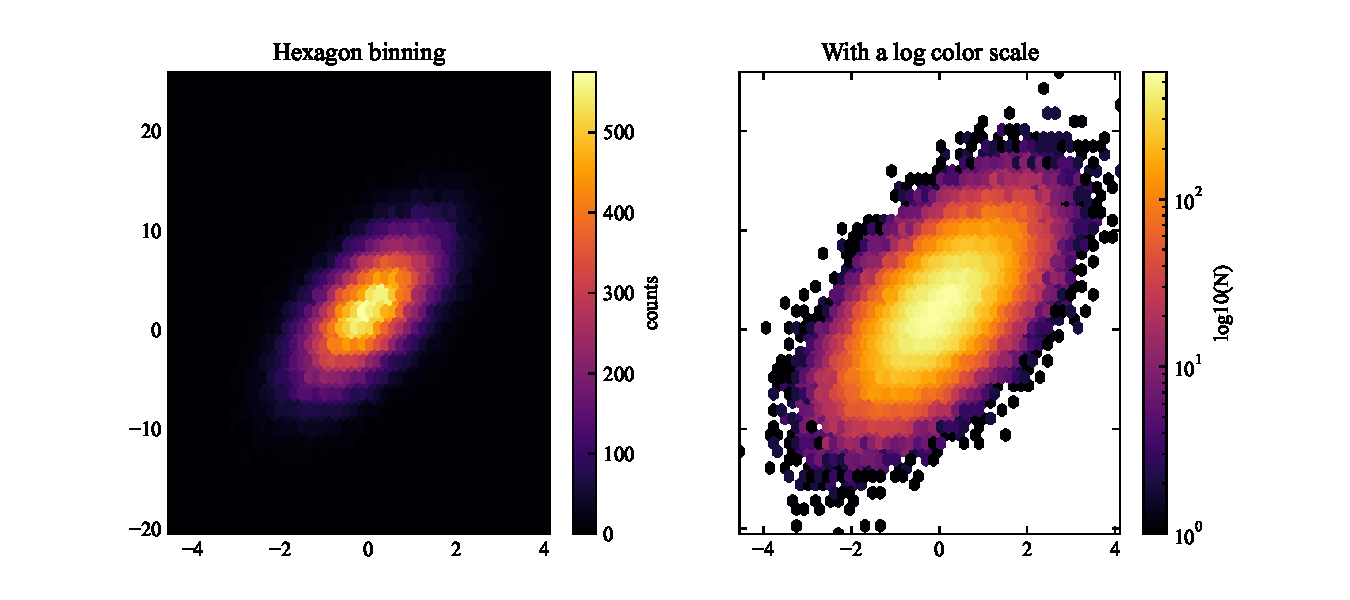
\includegraphics[width=1\textwidth]{figures/hexbin.pdf}
	\caption{六边形分bin图}
	\label{fig:hexbin}
\end{figure}
\begin{figure}[!htp]
	\centering
    \begin{subfigure}{0.45\textwidth}
        \centering
	    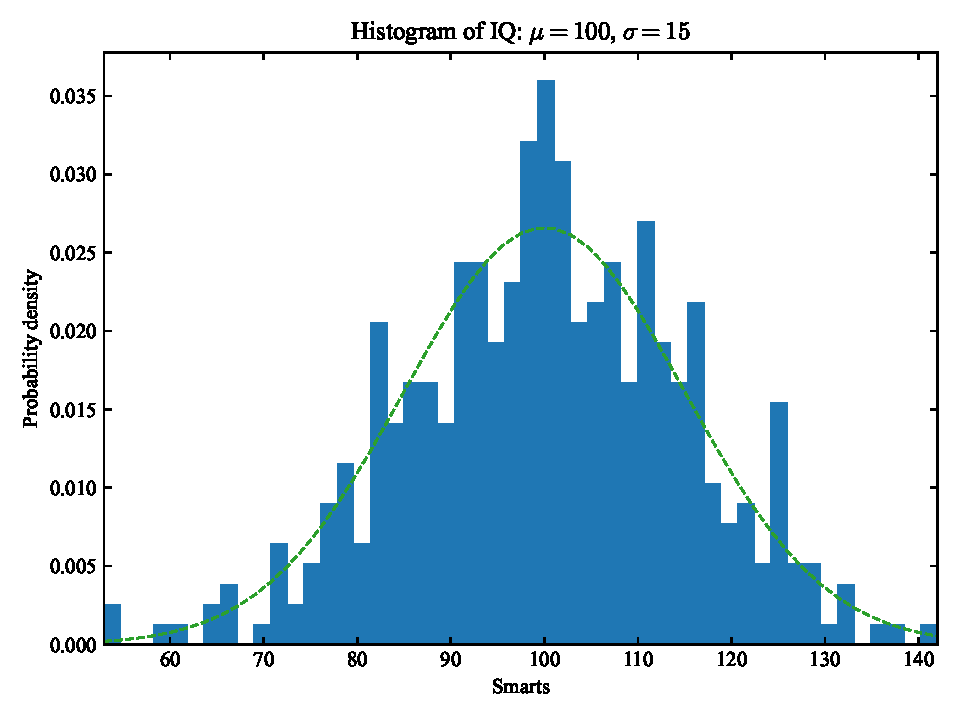
\includegraphics[width=1\textwidth]{figures/histogram.pdf}
	    \caption{柱状图}
    \end{subfigure}
    \begin{subfigure}{0.45\textwidth}
        \centering
	    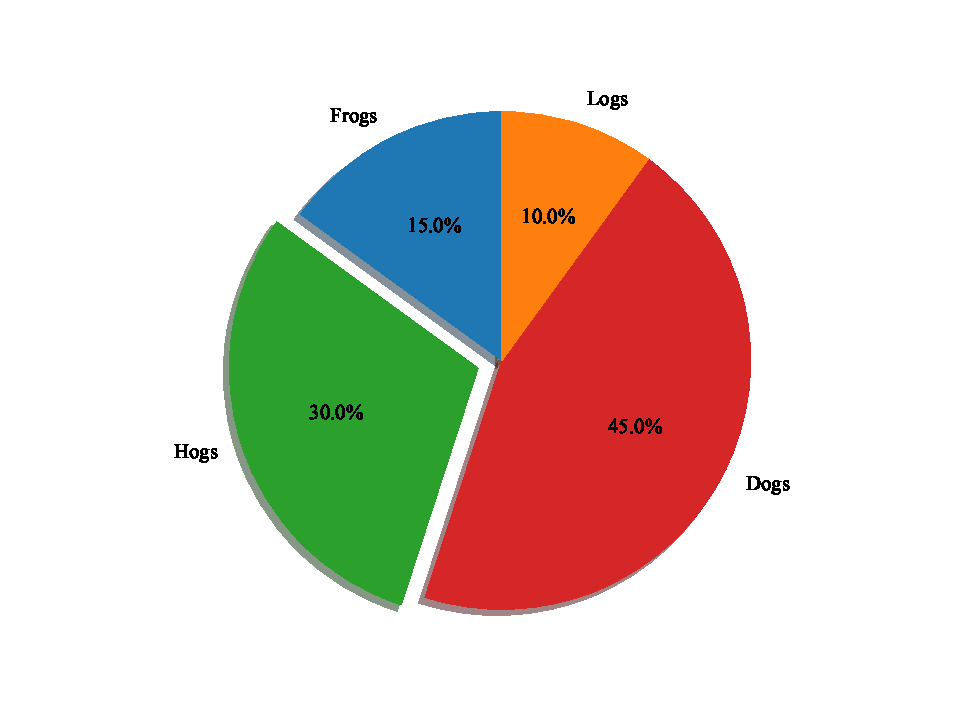
\includegraphics[width=1\textwidth]{figures/piechart.pdf}
	    \caption{饼状图}
    \end{subfigure}
    \caption{子图示例}
    \label{fig:subfig}
\end{figure}

插图的引用示例:\ref{fig:hexbin}是普通插图。

\section{表格示例}

文中的表格建议使用\texttt{table}环境里嵌套\texttt{tabular}环境,简单的表格样式一般采用三线表。
\begin{table}[!htp]
    \caption{2022年北京冬奥会奖牌榜}
    \label{tab:01}
    \centering
    \begin{tabular}{ccrrrr}
        \hline
        总排名 & 国家/地区 & 金牌 & 银牌 & 铜牌 & 合计  \\ 
        \hline
        1 & 挪威 & 16 & 8 & 13 & 37\\
        2 & 德国 & 12 & 10 & 5 & 27\\
        3 & 中国 & 9 & 4 & 2 & 15\\
        4 & 美国 & 8 & 10 & 7 & 25\\
        5 & 瑞典 & 8 & 5 & 5 & 18\\
        6 & 荷兰 & 8 & 5 & 4 & 17\\
        7 & 奥地利 & 7 & 7 & 4 & 18\\
        8 & 法国 & 7 & 2 & 5 & 14\\
        9 & 俄罗斯奥林匹克委员会\tablefootnote{俄罗斯由于被禁赛,不能以国家名义参加奥运会,不能使用国旗和国歌。因此俄罗斯代表团绕过禁令,以俄罗斯奥委会(Russian Olympic Committee)的名义参赛,以俄罗斯奥委会的会旗作为代表团的团旗,以柴可夫斯基的《第一钢琴协奏曲》作为团歌\cite{ROC}。} 
            & 6 & 12 & 14 & 32\\ 
        10 & 法国 & 5 & 7 & 2 & 14\\
        \hline
    \end{tabular}
\end{table}
这里需要注意,如果需要在表格内添加注释,请使用\texttt{tablefootnote}宏包的\texttt{$\backslash$tablefootnote}命令。如果要制作长表格,请使用\texttt{longtable}宏包的\texttt{longtable}环境。

表格的引用示例:\ref{tab:01}是2022年北京冬奥会奖牌榜。

\section{其他数学环境示例}

以下是本模版预设的数学环境示例:

\begin{assumption}[连续统假设]
    不存在一个基数绝对大于可数集而绝对小于实数集的集合。
\end{assumption}
\begin{axiom}[平行公理]
    若两条直线都与第三条直线相交,并且在同一边的内角之和小于两个直角,则这两条直线在这一边必定相交。
\end{axiom}
\begin{conjecture}[黎曼猜想]
    黎曼$\zeta$函数
    \begin{align}
        \zeta(s) = \frac{1}{1^s} + \frac{1}{2^s} + \frac{1}{3^s} + \frac{1}{4^s} + \cdots
    \end{align}
    非平凡点的实数部分是$\frac{1}{2}$。
\end{conjecture}
\begin{definition}[定义的定义]
    对一个概念或者词或者词组的定义是描写其内涵,即描写其所有和仅有的元素的共有特征。其外延是所有这个概念、词或者词组包含的事物。
\end{definition}
\begin{example}
    举个栗子。
\end{example}
\begin{exercise}
    TiMi,发出学习的声音。
\end{exercise}
\begin{lemma}[欧几里得引理]
    如果一个正整数整除另外两个正整数的乘积,第一个整数与第二个整数互质,那么第一个整数整除第三个整数。
\end{lemma}
\begin{problem}
    花儿为什么这样红?
\end{problem}
\begin{proposition}
    通过一个不在直线上的点,有且仅有一条不与该直线相交的直线。
\end{proposition}
\begin{theorem}[诺特定理]
    对于每个局部作用下的可微对称性,存在一个对应的守恒流。另言之,每个连续对称性都有着相应的守恒定律。
\end{theorem}
\begin{corollary}
    推论往往在定理后出现。如果命题B能够被简单明了的从命题A推导出,则称B为A的推论。
\end{corollary}
\begin{solution}
    这个问题无解。
\end{solution}
\begin{proof}
    因为爱情,不会轻易悲伤,所以一切都是幸福的模样。
\end{proof}

\section{代码示例}

在论文中插入代码,我们使用的是\texttt{listings}宏包的\texttt{lstlisting}环境,如:
\begin{lstlisting}[language=python]
import numpy as np
import matplotlib.pyplot as plt

# Fixing random state for reproducibility
np.random.seed(19680801)

dt = 0.01
t = np.arange(0, 30, dt)
nse1 = np.random.randn(len(t))                 # white noise 1
nse2 = np.random.randn(len(t))                 # white noise 2
    
# Two signals with a coherent part at 10Hz and a random part
s1 = np.sin(2 * np.pi * 10 * t) + nse1
s2 = np.sin(2 * np.pi * 10 * t) + nse2

fig, axs = plt.subplots(2, 1)
axs[0].plot(t, s1, t, s2)
axs[0].set_xlim(0, 2)
axs[0].set_xlabel('time')
axs[0].set_ylabel('s1 and s2')
axs[0].grid(True)
 
cxy, f = axs[1].cohere(s1, s2, 256, 1. / dt)
axs[1].set_ylabel('coherence')

fig.tight_layout()
plt.show()
\end{lstlisting}
或\texttt{$\backslash$lstinputlisting}命令,如:
\lstinputlisting[language=Python]{codes/cohere.py}
建议代码不设置\texttt{caption}选项,也不要使用\texttt{$\backslash$ref}来引用,因为我没给代码环境设置中文标签 (> <)。

\section{参考文献}\label{sec:bibstyle}

\subsection{引用格式}

\begin{enumerate}
    \item 参考文献为论文中所有引文、引用观点以及对论文有重要影响和启发的文献;
    \item 参考文献按在论文中出现的先后依次排序;个别学科若通用该学科惯用的排序规范,可以例外;
    \item 参考文献内容一般排列在论文末尾 (论文篇幅较大且引用文献较多的,可在每章末尾注出),序码与论文加注处对应;
    \item 参考文献标注格式:
        \begin{enumerate}
            \item 期刊:[序号] 作者. 文章题目. 刊名, 出版年份, 卷号(期号): 页码
            \item 图书:[序号] 著者. 书名. 版次(2版以上). 出版地, 出版年份. 页码
            \item 研讨会论文:[序号] 作者. 文章题目. 会议名称. 地名. 国名. 月份. 年份. 卷号
            \item 学位论文:[序号] 作者. 论文题目. 博/硕士论文. 校名. 页码、
            \item 电子文献:[序号] 主要责任者. 电子文献题名. 电子文献的出处或可获得地址, 发表或更新日期/引用日期(任选)
        \end{enumerate}

    例如:
        \begin{enumerate}
            \item 这是一个期刊的引用\cite{LIGOScientific:2017zic};
            \item 这是一个图书的引用\cite{Rubakov:2017xzr};
            \item 这是一个研讨会论文的引用\cite{Tanikawa:2021+x};
            \item 这是博士论文的引用\cite{Migenda:2019xbm,HuangGuoYuan:2020},这是硕论文的引用\cite{Shojaeifar:2015csv,SongRen:2020};
            \item 这是电子文献的引用\cite{Piro:2021oaa,bilibili:read}。
        \end{enumerate}
\end{enumerate}

\subsection{参考文献引用说明}

参考文献的引用格式已经由\texttt{sysuthesis.bst}设置好了。引用时,请将引用信息编入\texttt{ref}文件夹的\texttt{refs.bib}文件中,语法要符合\hologo{BibTeX}格式,并在文中引用处使用\texttt{$\backslash$cite}命令。建议只使用\ref{tab:entrytypes}中的几种\hologo{BibTeX}条目类型(Entry Types)。
\begin{table}[!htp]
    \caption{本模版设置好的\hologo{BibTeX}字段类型}
    \label{tab:entrytypes}
    \centering
    \begin{tabular}{ll}
    \hline
    引用文献的类型 & Entry Types \\
    \hline
    期刊    & \texttt{article} \\
    图书    & \texttt{book} \\
    研讨会论文    & \texttt{conference} \\  
    博士论文    & \texttt{phdthesis} \\
    硕士论文    & \texttt{mastersthesis} \\
    电子文献   & \texttt{online} \\
    \hline
    \end{tabular}
\end{table}
请注意:\strong{如果引用的是中文文献,请再额外添加\texttt{language} 字段,并让它不为空,否者将输出英文引用格式}。例如,这是一个\texttt{article}条目类型的源代码:
\begin{lstlisting}
@article{ZhaoWen:2017twxjz,
    author={赵文 and 张星 and 刘小金 and 张杨 and 王运永 and 张帆 and 肇宇航 and 郭越凡 and 陈奕康 and 艾舜柯 and 朱宗宏 and WANG Xiao-ge and LEBIGOT Eric and 都志辉 and 曹军威 and 钱进 and 殷聪 and 王建波 and BLAIR David and JU Li and ZHAO Chun-nong and WEN Lin-qing},
    title={ 引力波与引力波源 },
    journal={天文学进展},
    language={中文},
    year={2017},
    volume={35},
    number={3},
    pages={316-344},
    month={1},
}
\end{lstlisting}
请点击\cite{ZhaoWen:2017twxjz}查看该期刊文章的引用效果。这是中文图书的引用效果\cite{Huang:2012hxwl}。

\section{注释}
注释:可以用“脚注”或“文后注”来标注引用著作中的一些观点和案例,但全文标注方式应统一,本文统一使用“脚注”\footnote{这里是注释内容。}。


% 结语
% !TEX root = ../main.tex
\begin{summary}

    任何有关本模版的问题以及建议,欢迎通过以下其一方式来联系我:
    \begin{itemize}
        \item 本模版的\href{https://jq.qq.com/?_wv=1027&k=eA9mGWmS}{\strong{企鹅交流群}},主要用于本模版的维护和交流;
        \item 我的个人\href{https://space.bilibili.com/326100515}{\strong{B站号}},常用,一般能很快看到消息;
        \item 我的\href{https://space.bilibili.com/326100515}{\strong{GitHub}}主页,不常用,主要用于本模版的最新版本发布。
    \end{itemize}
\end{summary}

% 参考文献
\makebib{ref/refs}

% 附录
\appendix
% !TEX root = ../main.tex
\chapter{标题}
\section{附录说明}
附录是正文主体的补充。下列内容可以作为附录:
\begin{enumerate}
    \item 攻读学位期间发表的(含已录用,并有录用通知书
    的)与学位论文相关的学术论文目录。
    \item 由于篇幅过大,或取材于复制件不便编入正文的材
    料、数据。
    \item 对本专业同行有参考价值,但一般读者不必阅读的
    材料。
    \item 论文中使用的符号意义、单位缩写、程序全文及有
    关说明书。
    \item 附件:计算机程序清单、软磁盘、鉴定证书、获奖
    奖状或专利证书的复印件等。
\end{enumerate}


% 后置部分
\backmatter

% 致谢,即后记
% !TEX root = ../main.tex
\begin{acknowledgements}
    后记是有关本论文情况的说明性文字,主要是交代编写过程,阐述作者的感想和体会,对有关单位或个人的致谢语等。

    本模版在编写的过程当中,遇到了不少问题,也参考了许多小组以及个人的工具和模版:
    \begin{itemize}
        \item 感谢\href{https://github.com/CTeX-org/ctex-kit}{\strong{CTex-kit}}提供了\LaTeX{}的中文支持,其开发的\href{https://ctan.org/tex-archive/language/chinese/ctex}{\strong{CTeX}}宏集在章节格式的排版上提供了很大的方便;
        \item 感谢\href{https://www.zhihu.com/people/sgcd-33}{\strong{白鸽坐飞机}}师兄,本模版在排版上主要参考了他的中山大学研究生毕业论文模板\href{https://www.overleaf.com/latex/templates/zhong-shan-da-xue-yan-jiu-sheng-bi-ye-lun-wen-mo-ban-sysupalte/kybsnywqbcdc}{\strong{SYSUpalte}};
        \item 感谢\href{https://github.com/sjtug/SJTUThesis}{\strong{SJTUThesis}}模板的制作小组和\href{https://github.com/nanmu42}{\strong{李振楠}}(\href{https://github.com/nanmu42/CQUThesis}{\strong{CQUThesis}}),本模版在编写文档类文件的过程中主要参考了他们的成果,获益匪浅;
        \item 感谢\href{https://www.ctan.org/author/daly}{\strong{Patrick W. Daly}},本模版在制作参考文献引用格式的样式文件时使用了他的\href{https://www.ctan.org/tex-archive/macros/latex/contrib/custom-bib/}{\texttt{custom-bib}}工具;
    \end{itemize}
    向你们致以真诚的敬意和由衷的感谢!
\end{acknowledgements}



\cleardoublepage
\end{document}